\documentclass{./llncs2e/llncs}
\usepackage{graphicx}
%%%%
\usepackage{fixltx2e}
%%%%
\usepackage{mathtools}
%%%%
\usepackage[nolist,nohyperlinks]{acronym}
%%%%
\usepackage[section]{placeins}
%%%% Maintain images and tables within their respective sections
\usepackage{float}
%%%%
\usepackage[utf8]{inputenc}
%%%% Declare that we are using utf8 encoding
\usepackage{listings}
%%%% Include package for listings

\pagestyle{plain}
%%%% Use a page style that has page numbers

% 
% Change the margins
% 
% \usepackage[margin=2.9cm]{geometry}

\begin{document}
	
%%%%% Remove title and author from TOC
% make a proper TOC despite llncs
\setcounter{tocdepth}{2}
\makeatletter
\renewcommand*\l@author[2]{}
\renewcommand*\l@title[2]{}
\makeatother
%%%%%
	
	
\title{A Browser-based Interactive Development Environment for Generative Design}

%\subtitle{Your Thesis subtitle}
\author{Pedro Alfaiate, pedro.alfaiate@tecnico.ulisboa.pt}
\institute{Instituto Superior Técnico}

\maketitle

%----------------------------------------------------
%NAVabstract
\begin{abstract}
	%User interfaces can be built using web pages.
	%With modern web standards they are no longer limited to server-generated web pages, they can be as flexible as desktop user interfaces.
	%As they are web pages, this also means that they can be used in any computer connected to the internet.
	
	With \ac{gd} architects use algorithms to describe their designs and leave the work of generating concrete instances to the computer.
	It is extremely helpful when the design has plenty of repetition and it is necessary to explore variations.
	The development of \ac{gd} designs is greatly simplified by \acp{ide} such as Dynamo or Rosetta that provide a framework for writing programs that represent the design.

	Unfortunately, these \acp{ide} are only available in the computers where they were installed and for specific \acp{os}.
	Web-based applications do not suffer as much from this as they are developed for web browsers that run in most \acp{os} and that can be accessed from anywhere. 
	Moreover, modern web standards allow web-based applications to provide user interfaces as rich as those available for desktop applications.

	In this report we will look at examples of both desktop and web applications and will use them as a basis for proposing a web-based \ac{ide} for \ac{gd}.
\end{abstract}
%----------------------------------------------------
%NAVkeywords
\begin{keywords}
web application, Generative Design, integrated development environment
\end{keywords}

\tableofcontents

%%%% Acronyms in the abstract have to be repeated.
\acresetall

%----------------------------------------------------
%NAVintroduction
\section{Introduction}
	%Introduce the power of programming.
	Many people have understood the power that comes from having a computer (or machine) doing the repetitive work and like so have adopted programming as a new tool.

	%Introduce the need for IDEs. Introduce the demand for IDEs.
	Expressing ideas or processes as programs requires the programmer to specify every detail of what he has in mind (sometimes too much detail).
	This is only possible with plenty of discipline from the programmer.
	He has to write the program in a programming language.
	He has to store it following a specific file structure.
	If he uses an \ac{api}, he needs its documentation for quick reference.
	He may have to compile the program in order to run it.
	The compiler might detect syntactical errors that have to be corrected.
	If he notices that the program is misbehaving, he has to find the reason, which normally involves starting the program and attaching a debugger to it.
	When he finds the reason, he has to make corrections and test the program.
	And so on and so forth.

	All of this demands time and effort from the programmer and all those small steps have to be learned and articulated by the programmer.
	It is an inevitably complex activity and the programmer's productivity and enjoyment suffers from it.
	This suggests that we should find a way of lifting some of the work from the programmer, and that is where \acp{ide} come in.

	\acp{ide} bring together all the tools needed while programming and automate all its small steps.
	They might do it so well that the programmer might forget that those steps still exist.
	We can imagine that novice programmers using these environments would simply be unaware of them.
	Programmers still have to write, run and debug their programs but they do so without wasting time performing all those steps.
	This has made \acp{ide} essential to the programming activity.
	
	%Go from software production IDEs to architecture specific IDEs.
	%Software development -> domain specific -> architecture specific
	There are \ac{ide}s dedicated to supporting software production, like Eclipse\cite{eclipse2007eclipse} and Visual Studio\cite{mvs2002mvs}.
	These \ac{ide}s support several programming languages and provide many tools needed for software production.
	They help programmers navigate big software projects and let them configure complex building processes.
	They also help them organizing the work on their software projects.
	
	What software production \acp{ide} do not do is help non-specialist use programming for specific domains.
	They are intended to be general purpose and to be used by professional programmers and like so have complex interfaces and assume users know how to program.
	If someone wants to make a small program to solve his problem he will want something more specific that is not as complicated to use.
	
	%IDEs domain specific.
	As an example, consider IPython and Impromptu, which are \acp{ide} that are intended for two specific domains.
	IPython helps scientists by providing them what is relevant to their work, such as automating gathering of data, transforming and visualizing it in order to draw conclusions.
	It integrates taking notes and programming.
	They no longer have to join the pieces of information into a single space since it is already done by the environment.
	Impromptu helps musicians to compose music procedurally.
	A musician using Impromptu does not have to generate a MP3 file and then play it to actually hear what his program produced.
	He just starts his program and hears it.

	In this case, programming is no longer the main activity, it is used as a way to make computers do something we want.
	The results and ways to visualize (or hear) them are integrated into the environment.

	%IDEs architecture specific.
	Following the trend of using programming in their work, architects started using programming to generate the 3D models of the buildings they are designing, a process called \acf{gd}\cite{terzidis2003expressive,Maeda:2001:DN:559503}.
	While using \ac{gd}, they develop algorithms that describe how a 3D model of a design is built; when parameterized, these algorithms can easily create different versions of the design; this in turn enables architects to search for a version that satisfies them.
	
	As with scientists and musicians, architects can benefit from having \acp{ide} specific to their programming needs.

	There are several \acp{ide} that make it easier to program for \ac{gd}. 
	First, some \ac{cad} software packages used by architects have support for \ac{gd} provided by a plug-in or a set of plug-ins, as Visual Lisp in AutoCAD and Grasshopper in Rhinoceros3D.
	Second, there are standalone programming environments like Processing\cite{reas2007processing} or Rosetta\cite{de2012modern}; the first is a programming environment for the visual arts and the second is an environment thought specifically for \ac{gd}.
	
	These \acp{ide} need to be installed which is a problem when the architect wants to make a \ac{gd} program for a quick experiment but doesn't have it installed in his computer.
	It can become worse if the \ac{ide} he wants to use does not support the \ac{os} of his computer.

	One way to solve this problem is to move the \ac{ide} to a web page which is then accessed with a web browser.
	With a web-based \ac{ide}, architects only have to access its web page and no longer have to worry about \ac{os} compatibility or about installing it.

	The results of \ac{gd} programs in architecture are 3D models so it is central for an \ac{ide} for \ac{gd} to be able to display 3D models interactively.
	This is also true for a web-based \ac{ide}.
	
	Web-based applications with 3D graphics are becoming common now that hardware acceleration is possible thanks to WebGL\cite{marrin2011webgl}.
	Applications such as Clara.io\cite{houston2013clara}, a 3D modeling application, GooCreate\cite{goocreate2015site}, a game engine paired with a game editor, and OpenJSCAD\cite{openjscad2015site}, a modeling language with a browser based program editor, are some examples.
	
	
%----------------------------------------------------
%NAVobjectives
\subsection{Objectives}
	The aim of this project is to provide architects and designers interested in creating 3D models with an environment that fosters the \acl{gd} approach while being accessible wherever there is a web browser and an internet connection.

	When architects look for an environment to program they are not looking for a software development \ac{ide} like Eclipse or Visual Studio because, as explained before, these are excessively complex \acp{ide}, aimed for professional programmers using industrial programming languages.
	On the contrary, what architects look for in an \ac{ide} is a simple interface that considerably simplifies the development of \ac{gd} programs written in the dynamic languages typically used in \ac{gd}. 

	The result of this project should:
	\begin{enumerate}
		\item Support the \acl{gd} approach.
		\item Be implemented as a web page.
		\item Be available from the internet.
	\end{enumerate}
	

%----------------------------------------------------
%NAVrelatedwork
\section{Related Work}
	%TODO Introduce related work section

\subsection{IDE for GD}
	Developing and maintaining large software systems is a complex task.
	To deal with this complexity, software developers have many tools at their disposal and many of them are software systems themselves.
	Things like generating diagrams from source code (like class hierarchy diagrams and control-flow diagrams), source code versioning and management, testing frameworks, issue trackers, refactoring tools, debuggers and code editors with syntax highlighting and code completion are some of them.

	Using all of these tools in conjunction can be a difficult task since the developer needs to know the specific way to use each of them, both separately and together.
	This difficulty gave rise to \ac{ide}s that integrate all of these tools in one user interface.
	The \ac{ide} connects all the tools together so that developers do not have to worry about it and thus decreases the difficulty of using them.
	Overall, \ac{ide}s decrease the complexity of developing large software.

	Reducing the complexity of developing large software makes one wonder whether \acp{ide} can do the same to people programming for other purposes, such as \ac{gd}.
	It is not as simple as showing them the \ac{ide} and hoping they will know how to use it.
	In all likelihood they will be scared off by the sheer amount of buttons and menus the \ac{ide} has.
	The amount of time they would need to learn how to use it would be too much and they would rather solve their problem without programming.
	All those buttons and menus would act as a barrier; a barrier that would obscure the power hidden behind it.
	
	Nowadays, architects are starting to use programming and, therefore, need an \ac{ide}. 
	In order to effectively use an \ac{ide}, architects need specialized \acp{ide} with tools adapted to their needs.
	Since they are not concerned with making programs as complex as the ones from software development, the \ac{ide} does not have to be as complex.
	Without this complexity, the \ac{ide} can then provide tools that make programming for \ac{gd} easier.
	Displaying 3D models, for example, is essential as most \ac{gd} programs are intended to produce 3D models.
	
	\ac{ide}s like Dynamo\cite{dynamo2015site} and Rosetta\cite{de2012modern} already provide this and have gone further.
	Apart from being able to display 3D models, they have expressive programming languages and mechanisms to show the relation between the program and its results.
	They also have means to transfer the results of programs to the \ac{cad} software normally used by architects.
	
	Developing a new \ac{ide} for \ac{gd} requires us to study such \ac{ide}s.
	We can also look at \acp{ide} from other areas where programming is less complex than in software development.
	For example, tech savvy musicians use computers in live performances as their instruments and take advantage of their programmability through \ac{ide}s like Impromptu.
	Designers and visual artists use Processing and its \ac{ide}, the \ac{pde}, to program for their projects.
	Others can use IPython to document and inform their experiments by using Python's many libraries.
	All of these provide inspiration for an \ac{ide} for \ac{gd} and deserve to be further discussed.
	
%Domain-specific IDEs.
\subsubsection{Impromptu.}
	Impromptu\cite{sorensen2005impromptu,sorensen2010programming} is a programming environment developed to explore manipulation of musical structure in live performance; an \ac{ide} for musicians and sound artists.
	
	%What is live-performance?
	In the case of Impromptu, live performance takes place as a musician programs algorithms that produce music in front of an audience.
	During his performance, he writes the program that produces the sounds and chooses the right moments to change it to move between different parts of the music.
	
	%What does it provide to support live-performance?
	To enable live programming Impromptu brings together four components: an audio synthesizer, a real-time scheduling engine, a Scheme interpreter and an \ac{ide}. 
	The first three components make up the runtime environment, responsible for producing the sound, while the last provides an user interface, where the musician writes programs and sends them to the runtime. 
	
	%Describe live programming experience of impromptu.
	As he sends code, the musician builds the algorithm that produces the music incrementally.
	\footnote{The code sent to the runtime can define/redefine functions or variables, and schedule audio or functions to be played or run later.}
	To be able to keep producing sound for the audience he can program simple patterns, send them to the runtime and then change them as he programs more elements to compose the music.
	As he adds more elements he can start to make small changes to some of them which will be immediately audible.
	
	The immediacy from program changes to audible ones also lets the musician experiment with new ideas.
	Similarly, someone doing \ac{gd} will also benefit from having this immediacy in his \ac{ide}.
	
	
\subsubsection{IPython.}
	IPython\cite{PER-GRA:2007} is a notepad-like environment (Fig. \ref{fig:ipython:notebook}) directed towards providing better, more straightforward scientific computing. 
	%\emph{It makes me remember Mathematica's notebooks.} 
	As its name suggests, IPython's main programming language is Python. 
	While Python is its main programming language, other popular programming languages can be used in IPython, particularly those popular in the scientific community like R, or Julia.
	\footnote{More language kernels can be found in IPython's github page: https://github.com/ipython/ipython/wiki/IPython-kernels-for-other-languages}
		
	\begin{figure}
		\centering
		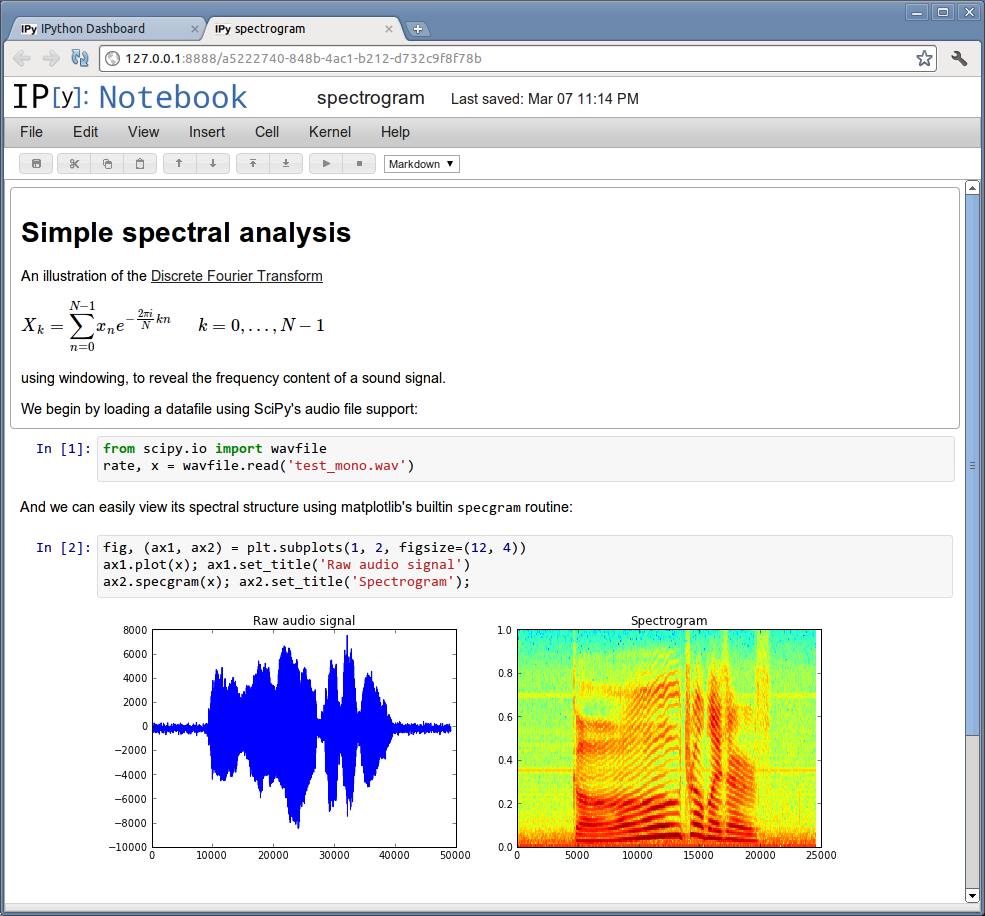
\includegraphics[width=0.8\textwidth]{img/ipython_notebook}
		\caption{An IPython notebook with rich text, mathematical notation, source code and results from executing such code.}
		\label{fig:ipython:notebook}
	\end{figure}
	
	One trend in its community, one that is supported by IPython notebooks, is to make results in publications more reproducible. 
	Instead of publishing a PDF or making a blog post, the authors write whole publications as IPython notebooks which then are shared and thus allow everyone to run their source code. 
	Having access to a working copy of the notebook, one can also experiment with it to better understand it, form own conclusions or find errors.
	
	%IPython architecture
	IPython was decomposed into execution kernels, a communication protocol and several front-ends. 
	As each type of component has a defined interface it is possible to implement new specialized components (a new front-end or a new execution kernel) that will integrate with those already implemented.
	
	%Why is it important? I cannot imagine designers using it.
	The style of producing notebooks in IPython is one that mixes programming, writing and exploring. 
	Interestingly, this style is also part of a designer's processes. 
	Like a scientist, the designer also has to do exploration of ideas (design ideas in his case), reach conclusions (finished designs) and share his work with others (fellow designers, clients, friends, blog readers). 
	Unfortunately, although IPython notebooks are natural tools for exploration, they do not provide domain specific functionality for architecture.
	
	
%Domain-specific IDEs for graphics, games, 3d modeling and Generative Design.
\subsubsection{Processing.}
	Processing\cite{reas2007processing} is a programming language and a development environment aimed at ``promoting software literacy in the visual arts and visual literacy within technology''.
	\footnote{Quoting www.processing.org, 9/Nov/2015.}
	
	Processing enables everyone to write programs that both draw to the screen and react to input from the user, like moving the mouse or pressing a key on the keyboard.
	It makes this possible by implementing most of the functionality (boilerplate code) that is required, like initializing the drawing surface.
	The programmer only has to implement the functionality that is specific to what result he wants to achieve.
	The code in Listing \ref{lst:simple:processing}, for instance, is what is needed to setup a drawing canvas, its background color and continuously draw a line from the mouse position to a point on the canvas.
	All the code is relevant to the purpose of the program.
	
	To use Processing's programming language, one needs to use the \ac{pde}.
	As shown in Fig. \ref{fig:proc:dev:env}, the \ac{pde} includes a text editor with syntax highlighting and runs Processing programs.

	\lstset{ %
		basicstyle=\tt\small,
		numbers=left,
		numberstyle=\tt\small,
		frame=lines,
	}
	\begin{lstlisting}[caption={A simple Processing sketch.},label={lst:simple:processing},float]
//Hello mouse.
void setup() {
	size(400, 400);
	stroke(255);
	background(192, 64, 0);
}

void draw() {
	line(150, 25, mouseX, mouseY);
}
	\end{lstlisting}
	
	\begin{figure}
		\centering
		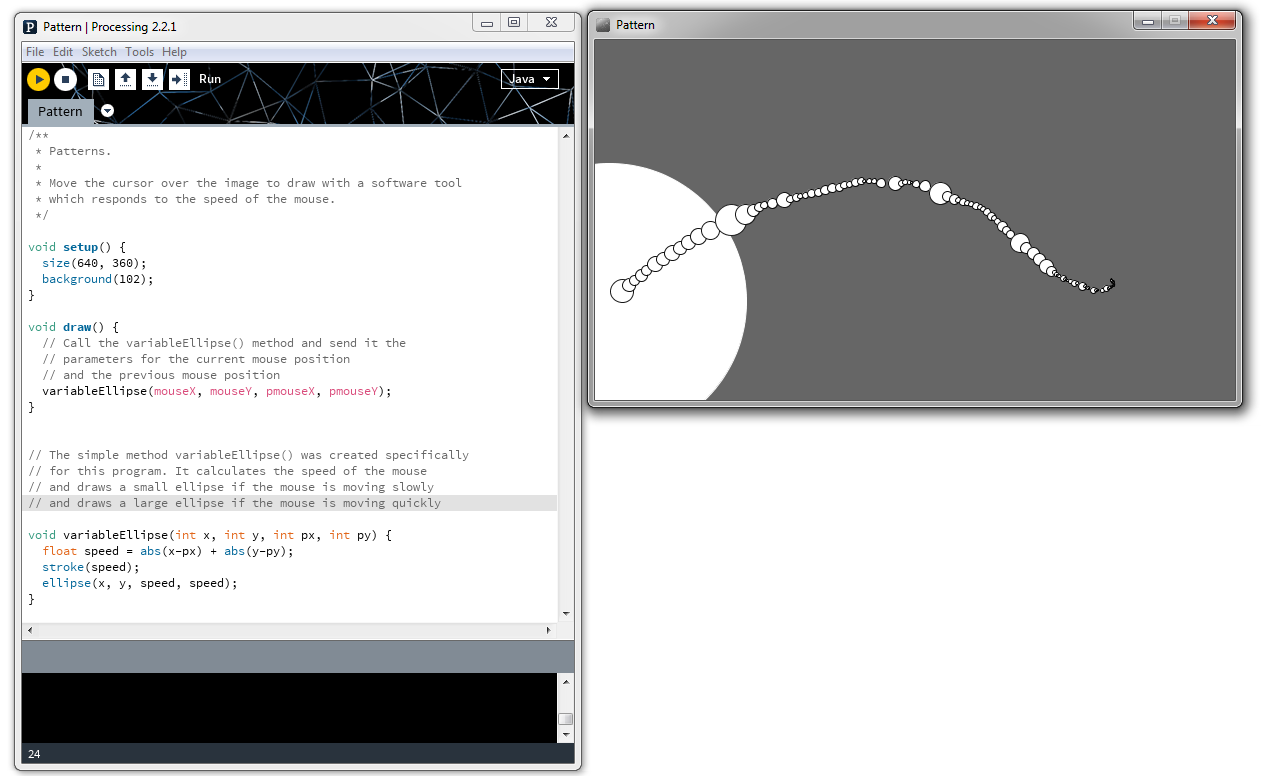
\includegraphics[width=1.0\textwidth]{img/proc_dev_env}
		\caption{On the left: The \ac{pde} displaying an example \emph{sketch} while it is being run. On the right: The drawing window to which the \emph{sketch's} instructions are applied.}
		\label{fig:proc:dev:env}
	\end{figure} 
	

\subsubsection{DesignScript.}
	%collections can be used everywhere one thing can be used
	%handling collections (replication guides, etc)
	DesignScript\cite{aish2012designscript} is a programming language that was designed to suit the needs of architecture related design and engineering.
	
	%DesignScript programming paradigms
	DesignScript uses concepts from multiple programming paradigms like object-oriented, functional and associative programming. 
	Entities have properties that can be either data or functions like in object-oriented languages; functions' most important role is to take some input and produce some output without producing side-effects like in functional languages; and dependencies among variables are retained like in associative languages.
	
	It supports both imperative (following instructions step-by-step) and associative (propagating changes in a dependency graph) control flows. 
	The programmer can choose to have portions of the code following one type of control flow and other portions following the other.
	
	%DesignScript primitives
	Being a domain-specific language for architecture, DesignScript includes not only primitives to make building 3d models but also operations from the rest of the architecture process such as energy related analysis and architectural elements (like creating or editing \ac{bim} families).
	%\emph{It may be better to provide a list of example primitives and operations.}
	
	Having modeling primitives close to those normally used in architecture software and combining several programming paradigms allows the designer to draw from knowledge about architecture modeling while empowering him to express the processes in which those primitives are used.
	
	%DesignScript editor(s)
	Editing DesignScript programs can be done either by writing or by creating a graph. 
	The graph is a more natural representation of the dependencies between the variables of the program when the associative paradigm is being used; it can also be viewed as a data-flow graph. 
	The written representation of DesignScript is a sequence of statements that specify the relationship between a variable and other variables; defining functions, using the imperative paradigm and reassigning variables is also possible; features that are less encouraged when a graph representation is being used.
	
	DesignScript is used in several environments. 
	These include a textual editor in Autodesk AutoCAD (Fig. \ref{fig:ds:autocad}), a dedicated graph editor called DesignScript Studio (Fig. \ref{fig:ds:dsstudio}) and later Dynamo (Fig. \ref{fig:ds:dynamo}). 
	Both DesignScript Studio and Dynamo use graph based program editing.
	
	\begin{figure}
		\centering
		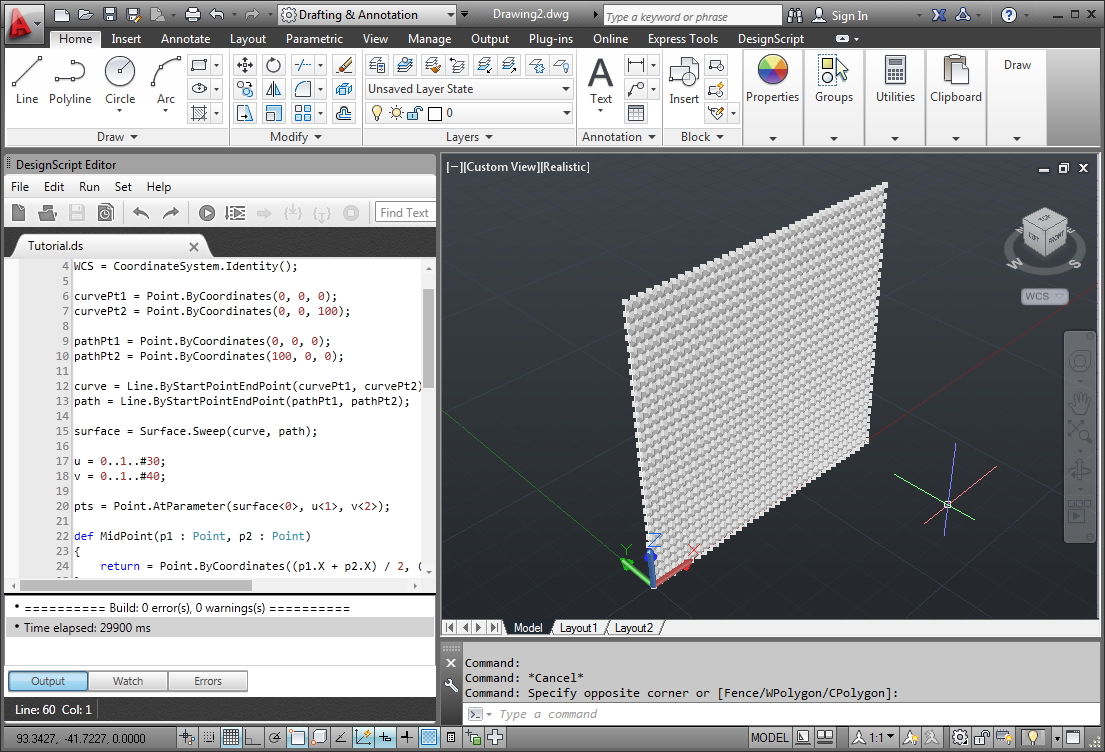
\includegraphics[width=0.8\textwidth]{img/ds_autocad}
		\caption{A DesignScript program being edited in a special text editor inside AutoCAD. This text editor provides auto-complete and a debugger.}
		\label{fig:ds:autocad}
	\end{figure} 
	
	\begin{figure}
		\centering
		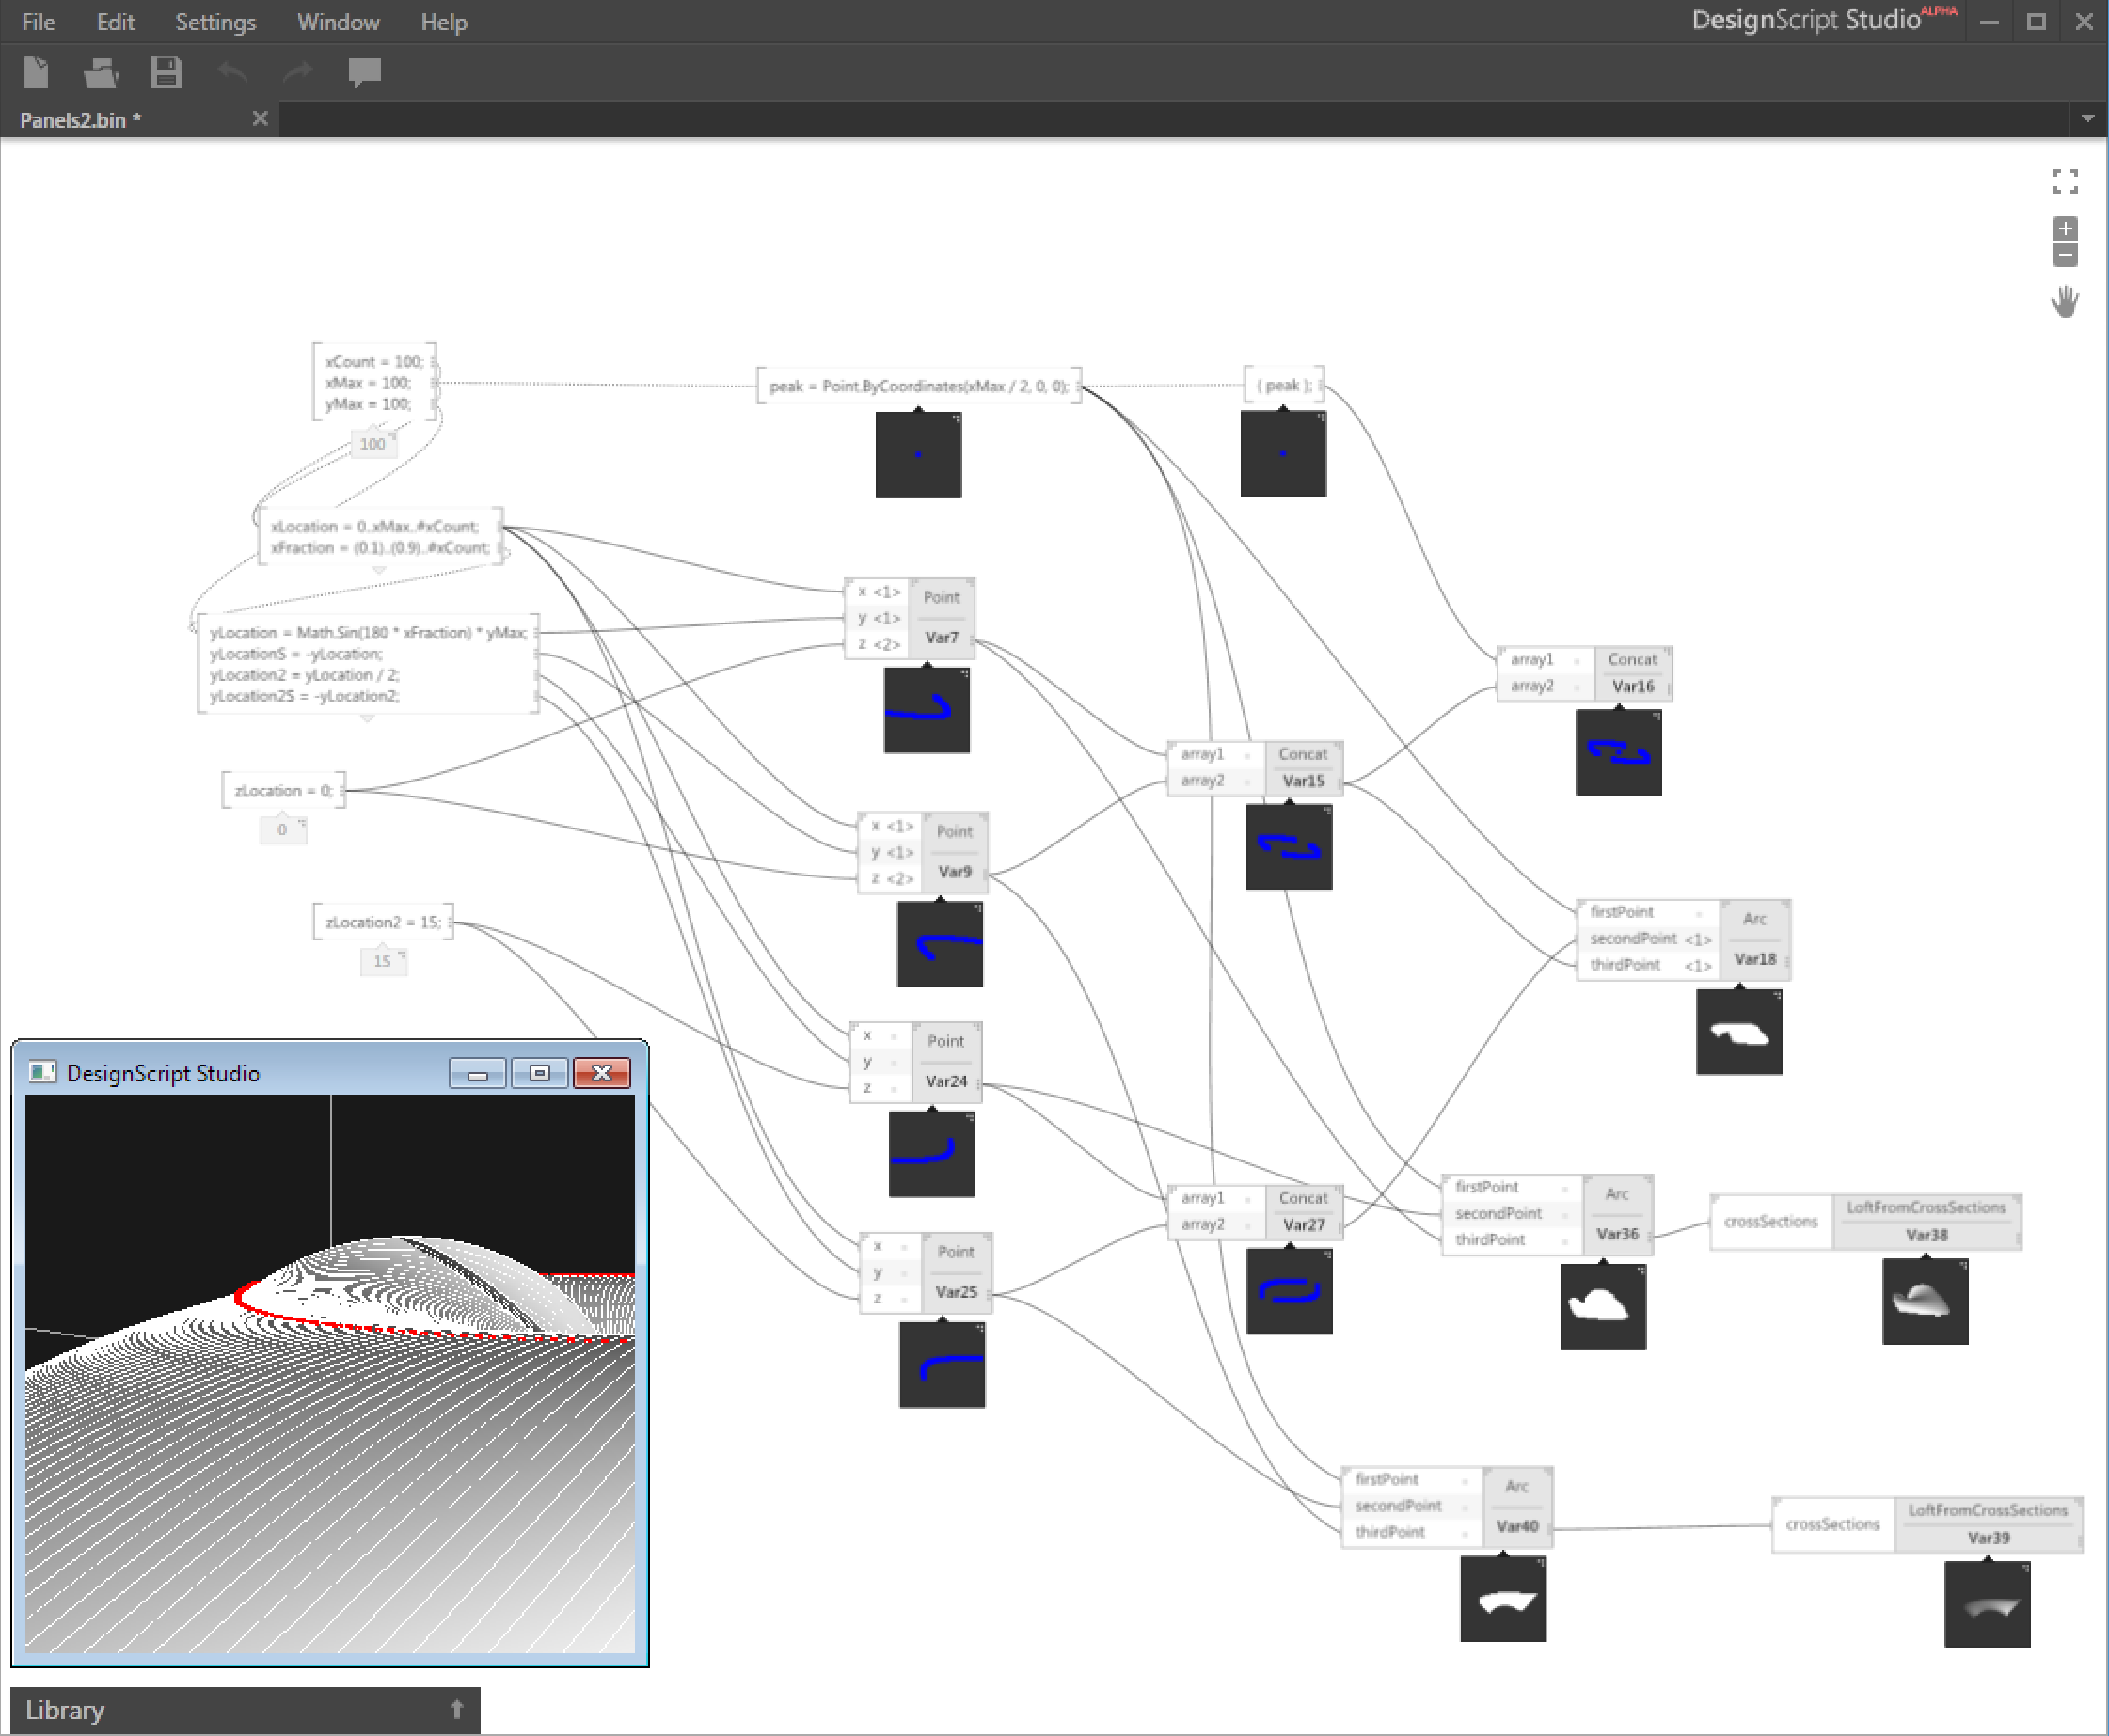
\includegraphics[width=0.8\textwidth]{img/ds_dsstudio}
		\caption{A DesignScript program as a graph in DesignScript Studio. Each node can display a preview of its results. To the bottom left corner is a preview of the whole program results and a folded library tab. The library tab contains everything that can be used in the program.}
		\label{fig:ds:dsstudio}
	\end{figure} 
	
	\begin{figure}
		\centering
		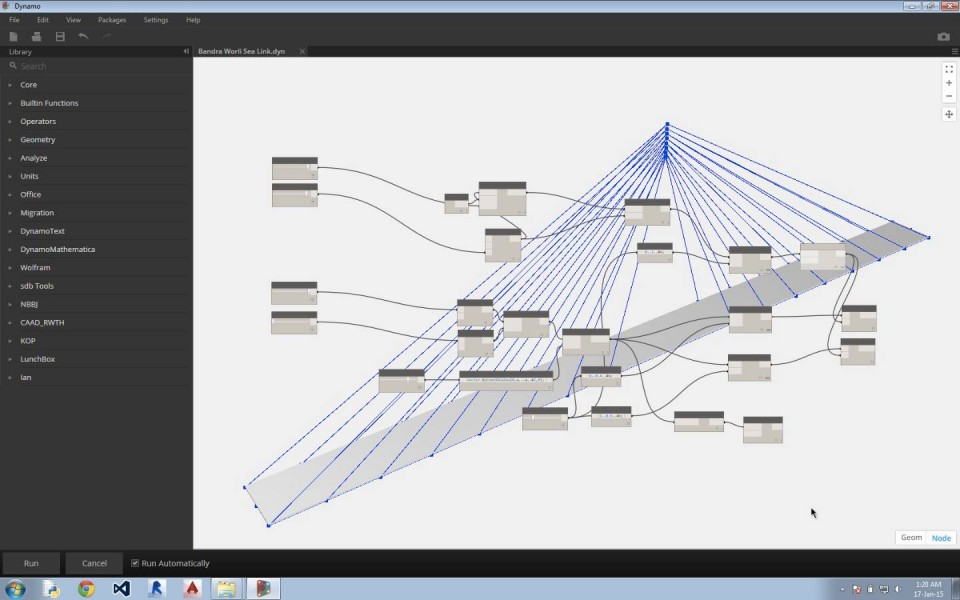
\includegraphics[width=0.8\textwidth]{img/ds_dynamo}
		\caption{Another DesignScript program as a graph in Dynamo. Like in DesignScript Studio a preview of the result of the program is displayed. A contrast is that there is only one preview ``canvas''; the preview from selected nodes is highlighted.}
		\label{fig:ds:dynamo}
	\end{figure} 
	
	Debugging DesignScript programs depends on the environment being used. 
	The textual environment allows to follow the execution of the program step-by-step while also supporting watches and breakpoints. 
	The graph-based environments allow highlighting and listing results of each node. 
	Both the textual and the graph-based environments provide a preview of the execution of programs.
	
	%Editing a DesignScript program is usually done in its dedicated development environment. DesignScript development environment provides auto-complete and debugging capabilities both of which are common features among programming environments.
	
	%DesignScript history
	DesignScript was later used as the scripting language of Dynamo, integrated with Autodesk Revit, where programs are edited as data-flow graphs. 
	DesignScript was also integrated into Autodesk AutoCAD. 
	A standalone node-based DesignScript editor was also made, it was called DesignScript Studio.
	
	%It is a multiple paradigm language supporting both imperative and associative programming. At any given point in a DesignSript program, the execution is either being controlled imperatively(following instructions step-by-step) or associatively(propagating changes in a dependency graph). It also uses object-oriented concepts; entities are objects with properties and methods; each object has its own properties and methods;
	%
	%One way DesignScript tries to succeed is to integrate various ways of modeling into the design process. These various ways of modeling are direct-manipulation mode present in any 3d modeling application, the associative mode present in many visual programming environments and the 

\subsubsection{Rosetta.}
	Rosetta\cite{de2012modern,lopes2011portable}, shown in Fig. \ref{fig:rosetta:ex}, is a platform for \ac{gd}.
	It grew from the desire to give the freedom to architects using the \ac{gd} to write their programs using the programming language they want and to easily switch where it takes effect.
	
	\begin{figure}
		\centering
		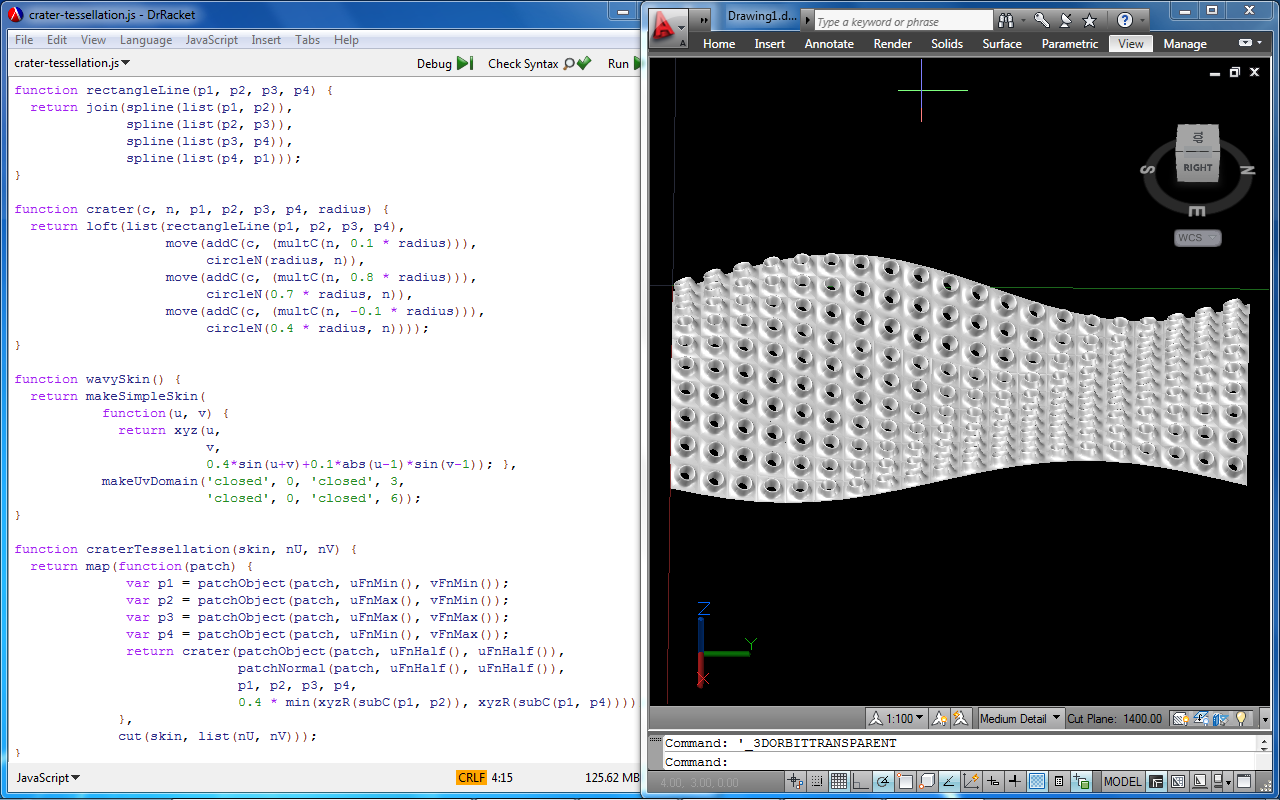
\includegraphics[width=0.8\textwidth]{img/rosetta_js_autocad}
		\caption{A Rosetta program in DrRacket (left) and AutoCAD displaying its results (right). The program is written in Javascript.}
		\label{fig:rosetta:ex}
	\end{figure} 
	
	%TODO simplify rosetta
	%%%%
	Its authors argue that most environments for \ac{gd}, developed for a specific \ac{cad}, do not provide portability of programs developed inside them.
	They also argue that \ac{vpl}s, based on data-flow graphs, do not provide good abstraction mechanisms; programs on such languages are therefore hard to understand and modify.
	
	It is also stated that industrial programming languages, like C, C++, Java and C\#, do not provide domain-specific abstractions from \ac{gd} and so they are inadequate.
	
	A survey of the most used \ac{gd} systems showed that the most popular \ac{tpl}s for \ac{gd}, like AutoLisp, RhinoScript, and GDL, are old, provide little domain-specific features and make it difficult to define them\cite{de2012modern,leitao2012programming}.
	It also showed that \ac{vpl}s for \ac{gd}, like Grasshopper and GenerativeComponents, enforce a very restricted programming paradigm and programs scale poorly with size and complexity, making them suitable only for small throwaway prototypes. 
	It also showed that \ac{cad} applications, being based on direct user interaction and imposing their own programming environments and languages, lock their users to the application's product family and make it difficult to achieve correctness, performance and portability.
	%%%%
	
	The design principles followed by Rosetta are:
	\begin{itemize}
		\item portability: program independence from \ac{cad} applications; enabling reuse of programs across different \ac{cad} application communities.
		\item parametric elements: do not require designers to manually transform parametric elements into geometric shapes \ac{cad}s understand.
		\item functional operations: operations do not consume their arguments; do not leak \ac{cad} implementation details into \ac{gd} languages.
		\item dimension independent operations: uniform, predictable treatment of shapes of different dimensions.
		\item algebra of sets: shapes as point sets in three dimensional sets; support for operations on sets.
		\item algebraic equivalences: to handle support discrepancies of set operations across \ac{cad}s and for optimization.
		\item traceability: between the parts of the program and their results.
		\item immediate feedback: to changes made to the program and its input.
	\end{itemize}
	
	A modern programming environment for \ac{gd} should:
	\begin{itemize}
		\item be pedagogic
		\item provide domain-specific features
		\item provide multiple Programming Languages
		\item provide multiple \ac{cad} applications
	\end{itemize}
	
	Generative Design needs:
	\begin{itemize}
		\item Portability
		\item Mathematical and geometric strictness
		\item Correlation between programs and models
		\item Multiple paradigms and techniques
		\item Modern and pedagogic system
	\end{itemize}
	
	It enables this by providing several front-end programming languages and several back-ends which take the results of the program. 
	The programs written in a front-end language are compiled into an intermediate language which then translates its semantics to the selected back-end\cite{lopes2011portable}.
	
	Some front-ends supported by Rosetta are AutoLisp, Javascript, Racket and Python; some of the supported back-ends include Autodesk AutoCAD, Autodesk Revit, Sketchup, Rhinoceros 3D, TikZ and OpenGL.
	
	%Rosetta has been extensively used for teaching programming to architecture students at \ac{ist}. 

\subsubsection{Learnable Programming.}
	Writing a program in a programming language can be difficult even if it was designed to be easy to use. 
	When a programming language is coupled with an environment specifically designed for it the programming experience improves drastically. 
	In his essay\cite{victor2012learnable}, Bret Victor described design principles over systems for learning programming.
	
	The programming language and the programming environment are essential parts of the programming experience.
	The programming language allows the programmer to express himself in a clear, specific way; the programming environment allows him to write programs and understand what they actually do.
	
	%TODO clarify what PL must do
	%%%%
	
	%%%%
	Programs written in the programming language need to reflect something from the programmer that is useful for programming.
	They should be about things the programmer can identify with (something that he knows); should allow him to talk about different parts of the problem separately; should allow him to bring those parts together; and should be readable.
	
	The environment needs to help understand the meaning of the parts of the program; understand the way the program execution evolves; understand the way the state of the program evolves; assemble parts together; and create new parts from existing ones.
	It should make these things easy to do, after all these can be done by the programmer himself if he is willing to.

\subsection{Moving to the Web}
	Web browsers did not start as feature-rich and performant as they are now.
	They started as hypertext browsers that made it easier to read hypertext.
	They could display images and text and could jump from page to page by following hyperlinks or following URLs.
	Only with the development of new features and the demand for more performance did they slowly get into the shape they are now.

	The number of devices connected to the internet is big enough to say that internet access is almost ubiquitous.
	People no longer have to rely on a single device because many of the things they do on that device can be migrated to the internet as distributed systems.
	If viewed this way, devices can become interfaces to distributed systems on the internet and people can start to use any device to access those distributed systems.

	There must be a platform to support (as in display) such interfaces and Web browsers are a good possibility.
	Almost any of these devices have web browsers.
	These not only include the traditional desktop and laptop computers but also the new smartphones, tablets, gaming consoles, smart appliances and the list goes on and on.

	Web browsers enable devices to connect their users to the \ac{www} and in many cases to the rest of the internet, as \ac{www} is often used as an interface to services on the internet.
	Some of those interfaces are as simple as a series of web pages generated by the service as they are used and some are as complex as pages interactively evolving with user input while at the same time exchanging information with many servers.
	Most blogs are examples of the first, technically simple, and most social networking sites are examples of the second, technically complex.
	All of these have forced web browsers to evolve into a performant, feature-rich platform.
	The extent of their performance and features makes them even capable of hosting desktop applications from code editors to video games (without plugins like Adobe Flash).

	%TODO do not begin with "And"
	And this has caught on.
	More and more people are replacing their desktop applications with web based ones.
	Web browsers are effectively replacing \ac{os}-level applications.
	And this also comes as an advantage for developers as the browser acts as an uniform platform across all different devices they want to develop for.

	It is in this time where web browsers are so capable that it becomes possible to develop a \ac{gd} \ac{ide} for the web.
	In the next sections, we describe a few relevant \ac{ide} that run on web browsers.

%Inspiration from anything about IDEs.
\subsubsection{LightTable.}
	LightTable\cite{lighttable2015site} is a code editor for the Clojure programming language[6] and is an example of a desktop application that uses Web technologies.
	More specifically, it uses node-webkit as its runtime allowing it to use the html layout engine for its user interface, to use Javascript as its programming language and to use node.js\cite{tilkov2010node} modules.
	LightTable is written in ClojureScript\cite{10.1109/MIC.2011.148}, a subset of Clojure that compiles to Javascript.

	%Disclaimer
	%Most of the features described here are only present in LightTable's several experimental versions. 
	%The release version's features are not what matters. 
	%The ideas behind the experiments are.

	%Why is LightTable relevant?
	%As of now, LightTable does not seem to be fulfilling its potential.
	LightTable uses the drafting table as its metaphor.
	\footnote{http://www.chris-granger.com/2012/04/12/light-table---a-new-ide-concept/ at Nov/2015.}
	The metaphor comes from looking at the way work is done in other fields of engineering, where engineers spread all materials relevant to their work over large tables, from tools to reference information. 
	Instead of displaying the contents of entire files, LightTable divides the code into meaningful units and displays them as small editors spread over the table's surface. 
	In one of its experimental versions, LightTable also supported displaying running programs in the table. 
	Fig. \ref{fig:lt:draft:table} shows an example of this metaphor.

	This metaphor has some resemblances to node-based programming environments. 
	The programmer still has to think of how to arrange what is on the table.
	What makes it different is allowing to choose what is on the table instead of having everything on it all the time.

	\begin{figure}
	  \centering
	  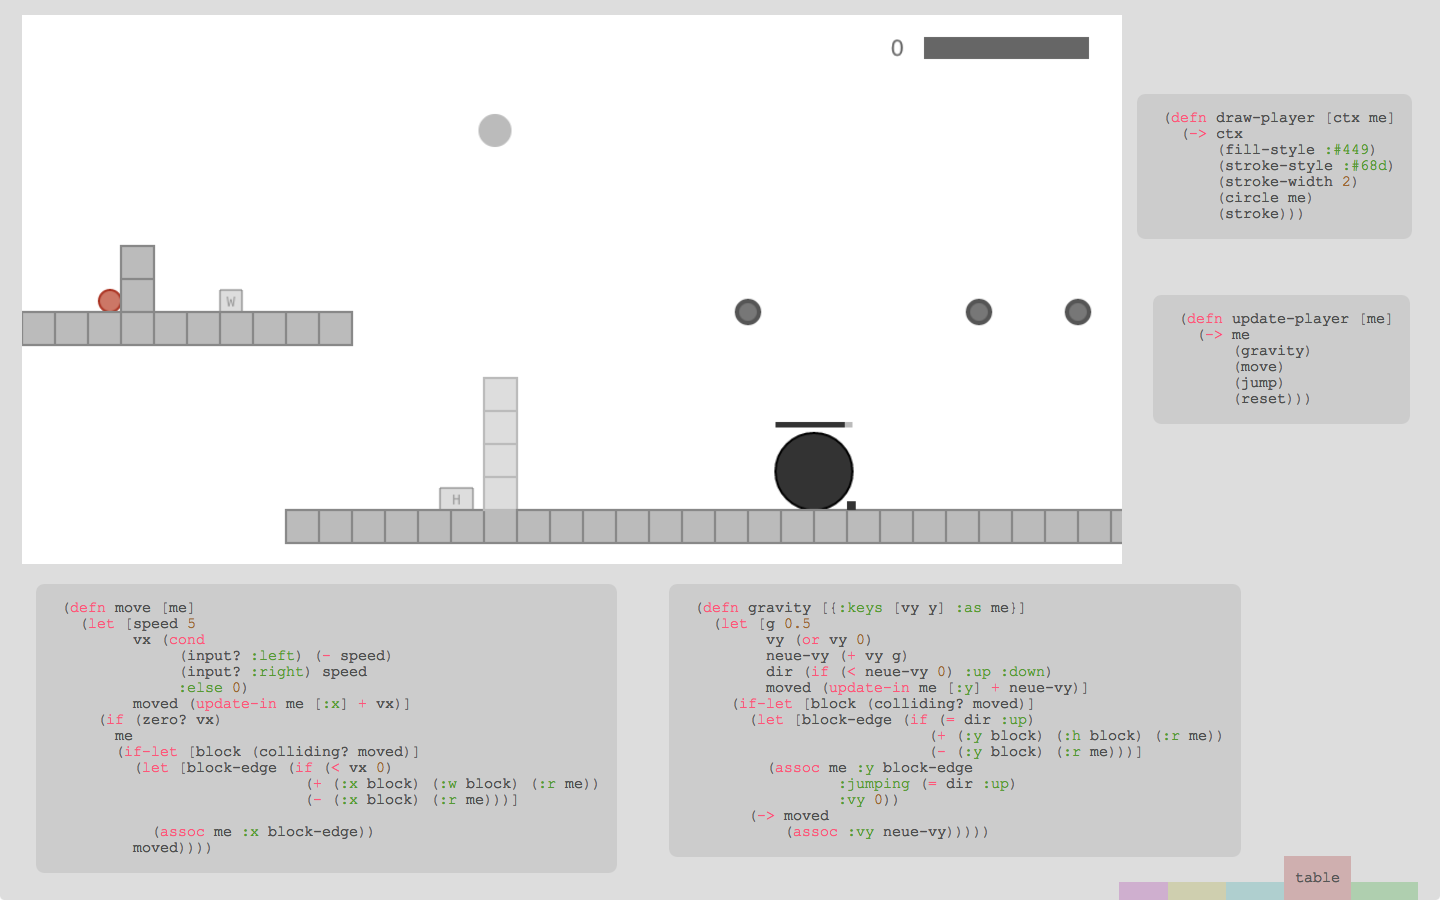
\includegraphics[width=1.0\textwidth]{img/lt_game_example__inv}
	    \caption{A prototype version of LightTable. A game is being run inside it while some of its code is displayed in separate editors.}
	  \label{fig:lt:draft:table}
	\end{figure} 

	%LightTable "function navigation"
	LightTable also helps navigating Clojure code bases.
	In Clojure, functions are defined inside namespaces and all Clojure definitions (functions, variables, macros) are stored in text files. 
	Navigating among definitions and the current namespace structure should not get in the way of editing code. 
	To make editing easier, LightTable provides a \emph{namespace browser} that eases finding functions and a \emph{code document} where functions can be added for editing without moving them out of their namespace or displaying entire files where they are defined. 
	Fig. \ref{fig:lt:clojure:table} shows an experiment where these two are used.

	\begin{figure}
	  \centering
	  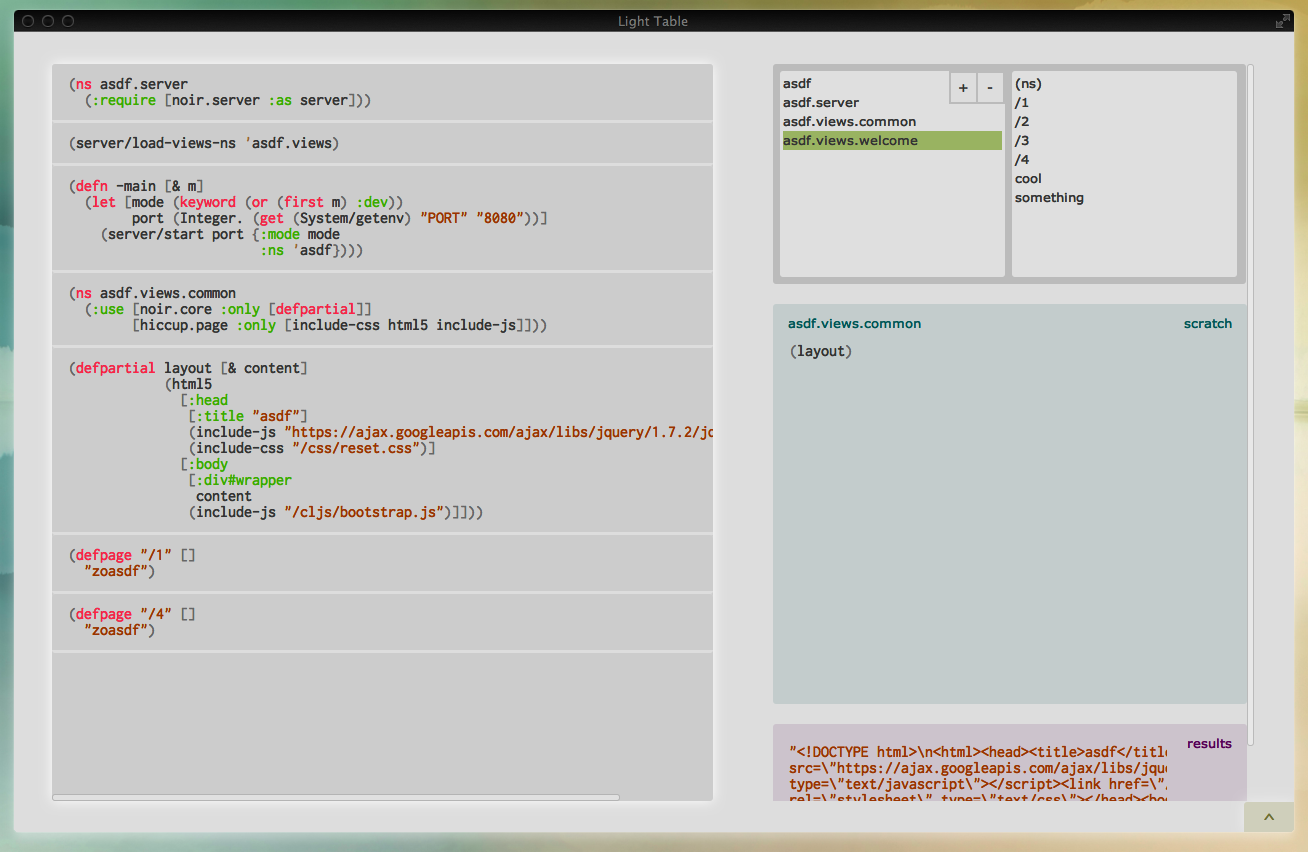
\includegraphics[width=1.0\textwidth]{img/lt_clojure_table__inv}
	    \caption{An experiment showing a \emph{code document} on the left and a \emph{namespace browser} on the top right.}
	  \label{fig:lt:clojure:table}
	\end{figure} 

	%LightTable "variable substitution"
	One interesting functionality of LightTable is its ability to show data flow in a function call. 
	Since the main purpose of a function is to transform its input data into its output data, it helps to see what happens to the data on each step of the function. 
	To achieve this, LightTable overlays variable values and return values, respectively, on each variable occurrence and expression of the function. 
	Fig. \ref{fig:lt:val:overlay} shows an example of such functionality. 
	This functionality is part of LightTable's \emph{instarepl}.

	\begin{figure}
		\centering
		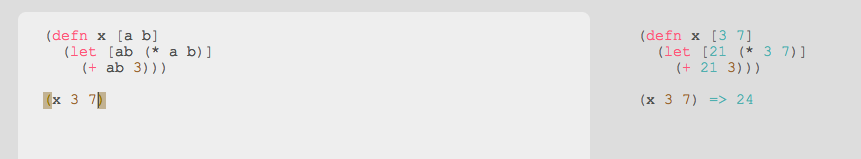
\includegraphics[width=1.0\textwidth]{img/lt_val_overlay__inv}
			\caption{An example of LightTable's value overlaying. The occurrences of the variables \emph{a}, \emph{b} and \emph{ab} were replaced with their values while evaluating the expression \emph{(x 3 7)}; the result of this expression is also overlaid.}
		\label{fig:lt:val:overlay}
	\end{figure}

	The main design pattern used in LightTable is the \ac{bot} pattern. 
	As described by one of its developers,\footnote{http://www.chris-granger.com/2013/01/24/the-ide-as-data/ at Nov/2015.} LightTable can be described as a set of \emph{Objects}, each having a set of \emph{Behaviors} and being tagged with a set of \emph{Tags}. 
	The \emph{Behaviors} describe how an \emph{Object} reacts when events are raised on it. \emph{Tags} are groups of \emph{Behaviors}. 
	When an event is raised on an \emph{Object} both its \emph{Behaviors} and those from its \emph{Tags} are notified.

\subsubsection{OpenJSCAD.}
	OpenJSCAD\cite{openjscad2015site} is a Javascript application (or rather, an application based on web technologies).
	It aims to provide the same functionality as OpenSCAD\cite{kintel2011openscad} but using Javascript as a base for its language. 
	Most of OpenSCAD functionality is implemented in OpenJSCAD. 
	Like OpenSCAD, it focuses on creating 3D models for 3D printing.

	To actually model in OpenJSCAD the user has to write a program in either OpenJSCAD's language or OpenSCAD's language.

	It is also possible to import 3D models from files commonly used for 3D printing like STL and AMF files.
	Upon import, the file's content is converted to a JSCAD program that produces the same model. 
	%(I do not see the point of doing this.)

	OpenJSCAD provides two user interfaces, one command-line interface and one graphical user interface as a web page.
	The first can be used for batch processing (running programs) while the second integrates an editor to edit a program and a 3D view for viewing the results of that program.

	%TODO fucking better explain dot syntax
	OpenJSCAD's language supports two syntaxes, one based on message passing (or method invocation/dot syntax) and one based on calling functions.
	Both of these syntaxes are already present in Javascript. 
	Many operations provided produce a new object and do not change their parameters. 
	This allows us to follow a functional programming paradigm and since there are fewer side-effects to know about it is easier to understand a program written using them.

	A problem that can arise while writing and testing jscad programs is that there is no help on getting the parameters for operations right and it is frustrating to spend more time than acceptable trying to understand why a certain operation is not producing the desired result. 
	This problem is even more relevant when most of the operations have multiple optional parameters and parameters that replace others. 
	Currently the only help available is OpenJSCAD's documentation (a tour on its functionality), the online community around OpenJSCAD and, since Javascript is the core of the language, web browsers' Javascript developer tools.

	There is also a problem using the function call syntax, namely its readability.
	The way function calls are written may not provide the flexibility needed for arranging the code in a readable manner. 
	This is especially true if a simple text editor is used. 
	%While assigning intermediary results to variables can help ``unnesting'' but it is sometimes inconvenient. 
	On top of this, OpenJSCAD is mainly just Javascript and like so Javascript's strange behavior about semicolon insertion is carried over. 
	%TODO fucking explain javascript semicolons

	%A good thing about being based on Javascript is that functions are first-class citizens.
	%It enables the programmer to specify parameters of functions as other functions 
	%Examples of this advantage can be found in \textbf{leitao abstract geometry n high order programming}.

	%For example, one can have a function describing how to make a building which receives functions describing how parts like balconies and windows are made as parameters.

	%Some functions in OpenJSCAD and their parameters.
	%function parameters result 
	%Each primitive has a lot of options on how to call it.
	%Its possible to round the edges of polyhedral primitives.
	%Non-polyhedral primitives are always converted to polyhedral approximations.

%----------------------------------------------------
%NAVarchitecture
\section{Architecture}
	In this section we discuss the architecture of the system we plan to develop to overcome the limitations of the systems previously described.

\subsection{Decomposing the problem}
	To better understand how to solve the problem of helping to make programs for GD, we decomposed it into several parts that can be more or less thought about and solved separately.
	
	\paragraph{The programming language.}
	One part that has to be set is \textbf{what is the language} used to make the programs.
	This aspect involves things like what control flow mechanisms are available, whether side-effects are allowed or not, and what is the syntax for each component of the language.
	It deals with how the language works.

	\paragraph{Help when writing and reading.}
	Another part is the \textbf{amount of help, documentation or reaction} the system has to support the user while he is thinking about and making the program.
	In the light of \cite{victor2012learnable}, the system should have good answers to the questions proposed on what is a good programming environment.

	\paragraph{Primitive operations.}
	Another part is the \textbf{implementation of the primitive operations} of the language like constructive solid geometry, lofts, sweeps and many other 3D modeling operations.
	Without them architects will not be able to make any Generative Design.
	One thing to keep in mind is that these operations have to be translated into other tools used in architecture.

	\paragraph{Documenting programs.}
	Another part is how the system lets users \textbf{document their programs}. 
	It is normal to forget how some part of the program works and so documentation is needed (or anything that is faster to understand than interpreting the program manually).
	The system could support having sketches juxtaposed to the program in addition to previews of results like those present in DesignScript Studio, Dynamo and Grasshopper. 
	It will also be useful to look at how current programming languages are usually documented. 

	\paragraph{Persisting programs.}
	%TODO persistence of programs
	Another part is the \textbf{persistence of programs} between usage sessions, in case the system crashes or even across multiple devices.
	In case of persistence between sessions, the user can close the browser or the tab at any moment, it would be useful to keep record of the current program in some way. 
	In case of persistence in case of crashes, if the user program itself crashed the page it should not be executed immediately to allow its retrieval or edition (as it could crash the page again). 
	With persistence of programs also comes the need for holding different versions of the same program. 
	These become useful as the user makes changes and wants to look back in time for some reason. 
	Maybe because he did not anticipate the need for something he deleted or maybe because he wants to see how his programs have progressed.

	\paragraph{Passing results on.}
	Another part is the way programs can be \textbf{applied to other modeling applications} used by architects.
	Without a way to do this the system is rendered useless as it can hardly be integrated into the architect's normal process. 
	Rosetta uses the concept of selecting a back-end, a specific interface to a modeling application. 
	After selecting a back-end for a modeling application, Rosetta connects to it and results of running the program are passed to the application. 
	The system could connect to Rosetta which would then connect to the application. 
	This approach requires the setup of a communication channel between the browser where the system is running and Rosetta. 
	The system could alternatively use a language that Rosetta already supports. 
	When the user wants to pass the result of the program to the application he only has to select the desired back-end and run the program inside Rosetta.

	%It should enumerate the various aspects of concern to be considered while making the solution. It may as well provide some alternatives to some aspects that are already known. These alternatives can refer to products already available.

\subsection{General Architecture of the Solution}
	%TODO more connection to requirements
	%Taking into account the aspects described above a version of the architecture of the solution was made.
	
	\begin{figure}
		\centering
		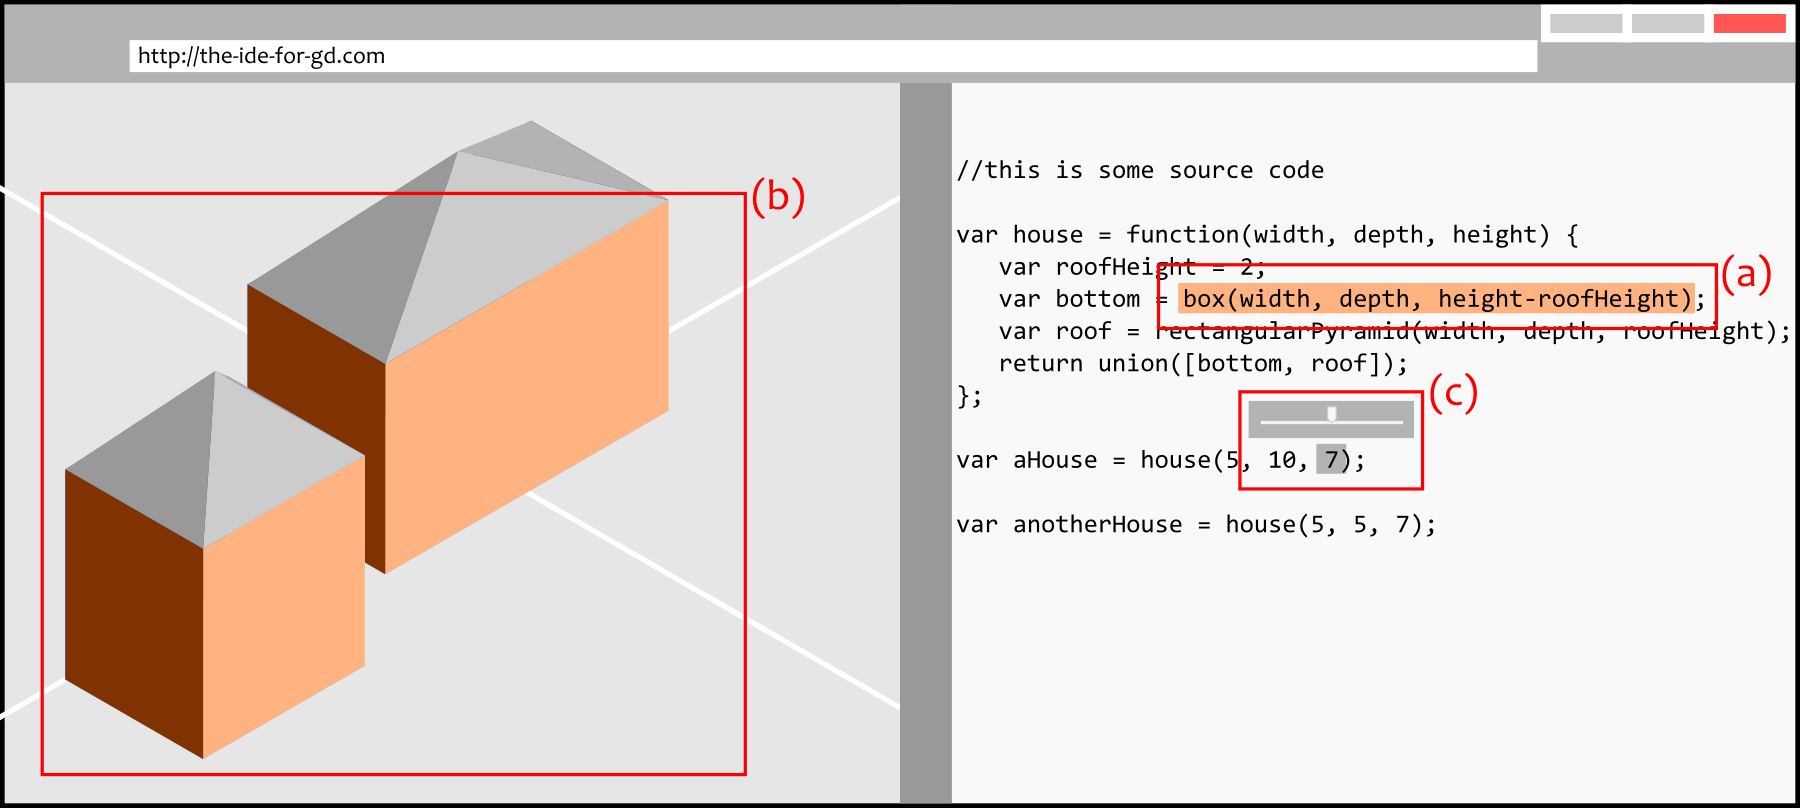
\includegraphics[width=1.0\textwidth]{img/ui_mock}
		\caption{A mock-up of the user interface. The results of the source code selected in (a) are highlighted in the 3D view of the results (b). (c) shows sliders can be used to change the value of constants.}
		\label{fig:ui:mock}
	\end{figure}
	
	The center of the \ac{ide} is composed by an editing environment, where source code is edited, and a visualizer, where results of running a program are visualized in 3D.
	Both of these are hosted within the web browser of the user and like so after the \ac{ide}'s web page is served to the browser it is no longer dependent on external computers.
	
	As starting ideas for features that will help users understand programs there is highlighting the 3D objects in the resulting scene that were ``affected'' by a part of the program (Fig. \ref{fig:ui:mock} (a) and (b)) and also letting users change the value of constants in source code using widgets, like sliders, to see their effects on results (Fig. \ref{fig:ui:mock} (c)).
	
	Interacting with programs and their results will only be possible if the \ac{ide} can display results or update them fast enough so a great part of our work will be in making sure it is.
	This may involve compromising the quality of the 3D scene that represents the results to get faster.
	
	Since there is no dependency on other machines, supporting program persistence and allowing the results of programs to get to other software are limited to what a web browser can do.
	Since web browsers allow some local storage to web pages, programs can be persisted there, at least temporarily.
	On the side of getting results into other software, without communication with the outside we are limited to either using a programming language supported by Rosetta or exporting to a widely supported file format.
	
	The architecture of the editing environment and the visualizer together with the program persistence module and the export module can be visualized in Fig. \ref{fig:gen:sol}.
	
	\begin{figure}
		\centering
		\includegraphics[width=1.0\textwidth]{img/gen_sol}
		\caption{A diagram of the architecture of the solution. Rectangles represent components, dashed rectangles represent where components will run and lines represent communication between components.}
		\label{fig:gen:sol}
	\end{figure}	

%----------------------------------------------------
%NAVevaluation
\section{Evaluation}
	To evaluate an \ac{ide} for \ac{gd} we will have to look at three different areas:
	its performance, its user experience or usability and its Generative Design capability.
	
	\paragraph{User experience / Usability.}
	For the system to be useful its users have to be able to use it.
	To assess that this is true we will do user testing.
	
	The tests will follow the line of asking users to complete a small \ac{gd} programming task followed by giving their opinion on how the usage experience went.
	We can complement those with questionnaires on the same subject and also by recording the usage sessions (which will also allow users to pinpoint their opinions).
	
	Only the editing environment will be tested this way since it is the only component that is used directly by architects.
	
	\paragraph{Generative Design capability.}
	The variety of results that can be made using the system is also important for its evaluation.
	The more \ac{gd} examples it can produce the better it is suited for use in a real-world scenario.
	A way to show how much variety of results it can make is to describe several examples that give glimpses of that variety.
	
	\paragraph{Performance.}
	The performance will have to be evaluated but more importantly its perceived performance, or responsiveness, will also be evaluated.
	As the \ac{ide} will be used by people, it is important that the interface responds quickly;
	in this case it will matter how much time it takes to see the changes made to a program appear on a view of its results.
	
	Performance will be evaluated by benchmarks to compare our solution with other \ac{gd} \ac{ide}s and also by measuring the frame rate of the viewer.
	The first measures raw performance and the second measures responsiveness.

\subsection{Proof-of-concept Prototype}
	A small prototype has been assembled to test the concept of a \ac{gd} environment in the browser.

	Like shown in Fig. \ref{fig:proto:3d:p:editor}, this prototype consists in a web page with a text editor and a 3D view.

	\begin{figure}
	  \centering
	  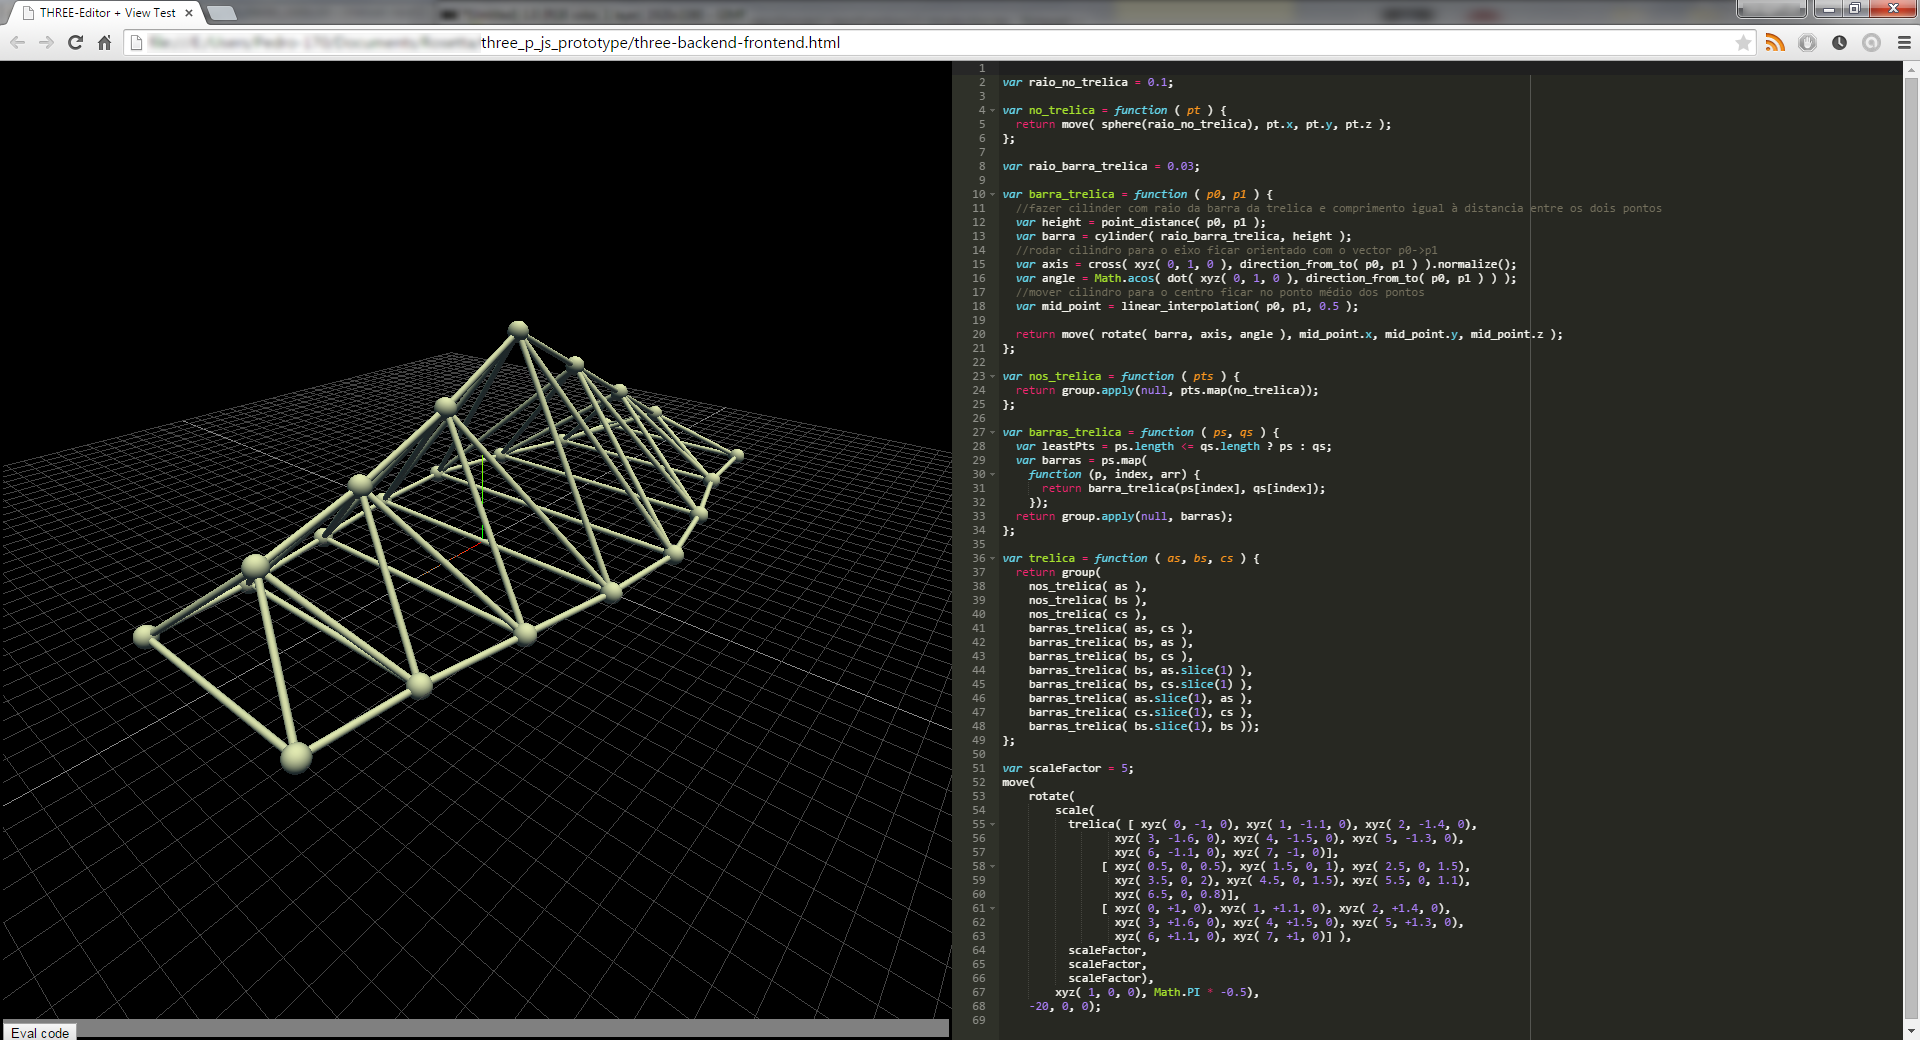
\includegraphics[width=1.0\textwidth]{img/proto_3d_p_editor}
	    \caption{The proof-of-concept prototype generating a truss. The right half contains the program used to generate the truss and the left half contains an interactive view of generated truss.}
	  \label{fig:proto:3d:p:editor}
	\end{figure} 

	The results of running the program inside the text editor are displayed through the 3D view. 
	When the program's text changes, it is rerun to reflect the changes in the 3D view. 
	This enables the prototype to provide immediate feedback to changes as long as they introduce visual changes to the result.

	The user can interact with the 3D view as if it contained a turntable.

	The programming language that is run by the prototype is Javascript with several functions added to produce 3D primitives (such as cubes or cylinders) and to manipulate those primitives (such as moving or grouping).

	The prototype is accompanied with example programs which were used to demonstrate it to a small group of potential users.

	The example programs try to emphasize functional programming techniques like using higher-order functions and minimal use of side-effects.

	The overall feedback we already obtained from the potential users was positive (they wanted to see it on a real application).

	The prototype is implemented using HTML, Javascript, CSS and also two Javascript libraries; the first, Ace\footnote{http://ace.c9.io/}, provides the text editor and the second, THREE.js\footnote{http://threejs.org/}, provides a high-level interface with WebGL rendering.

	With its naive implementation, the use of the prototype has already made one problem clear: always trying to run a program while it is being changed can lead to poor responsiveness or even permanent lockup of the interface, the usual cause being the increasing complexity of the program or the presence of infinite loops in the program. 
	This problem will have to be addressed in order to have a usable interface. 
	Some alternatives to solve the problem could be running the program asynchronously and retrieving the results afterwards or instrumenting the program so it could be run interleaved with interface handling and stopped if necessary.

%----------------------------------------------------
%NAVschedule
\section{Schedule}
	The schedule for the work concluding the thesis is presented in Fig. \ref{fig:schedule}.
	It has high-level tasks to convey the overall distribution of work for the thesis.
	
	\begin{figure}
		\centering
		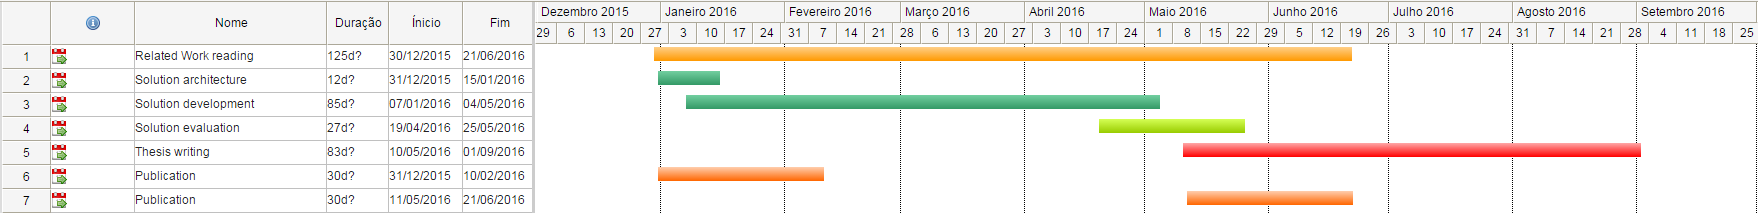
\includegraphics[width=1.0\textwidth]{img/schedule}
		\caption{This chart shows the overview of the work distribution.}
		\label{fig:schedule}
	\end{figure}
	
	The editing environment and the visualizer are the components where most implementation work is, since they are the central part of the architecture.
	The implementation of program persistence and result exportation will be in the background.
	As these implementation tasks are complex, they need to be further decomposed.
	
	During implementation we will test both user experience and performance of the system as part of its evaluation.
	
	Close to the end of the implementation we will start to assemble the thesis document and its defense.
	We will be writing parts of the document as candidates to publication in Architecture and Programming conferences.
	
	Some work has already been done.
	The proof-of-concept prototype is part of that work, more specifically part of the work on the editor.
		
	

%----------------------------------------------------
%NAVconclusions
\section{Conclusions}
	People making \ac{gd} need an \ac{ide} that is different from those used in software development. 
	Most of the time their programming projects are much simpler than the typical software development project.
	They also do not have as much programming knowledge as software developers.
	With this in mind it becomes clear that software development \acp{ide} (like Visual Studio or Eclipse) do not fit their needs.
	
	\ac{ide}s like Impromptu, IPython, Processing, DesignScript and Rosetta are examples of \ac{ide}s for programming purposes other than software development.
	They drop most of the functionality from software development \ac{ide}s  keeping only what is useful for beginners and adding new functionality that will help them while programming for their specific purposes.
	
	With the current state of web browsers it has become possible to host applications inside web pages. 
	Applications that in the past could only be executed by running a native executable can now be moved to web pages.
	LightTable and OpenJSCAD are examples of it.
	
	With the need for a different \ac{ide} for people doing \ac{gd} and the possibility of running applications in the browser, it is not only possible to build an \ac{ide} for \ac{gd} in the web browser but it is also advantageous for users.
	With it, they can quickly open up a web browser on its web page, start to write down their \ac{gd} ideas and immediately run them.
	
	To have a working \ac{ide} for \ac{gd} in the browser at least two components need to exist, a source code editor and a visualizer.
	This way people will be able to make programs and see their results with just a web browser.
	
	Making the user experience good will require special care.
	A particular element in making it is the overall responsiveness of the user interface and other is the amount of primitives available for \ac{gd}.
	
	In the future, a better solution for storing the programs users make and for running them in \ac{cad}s may be explored.
	
	%TODO even more independent conclusions
	
%----------------------------------------------------
%NAVappendix
\newpage
%\appendix
%\section{Appendix}
%\label{sec:attachments}

%----------------------------------------------------
%NAVacronyms
\begin{acronym}
	\acro{api}[API]{application programming interface}
	\acro{ide}[IDE]{integrated development environment}
	\acro{pde}[PDE]{Processing development environment}
	\acro{bot}[BOT]{Behavior-Object-Tag}
	\acro{bim}[BIM]{Building Information Model}
	\acro{ist}[IST]{Instituto Superior Técnico}
	\acro{gd}[GD]{Generative Design}
	\acro{repl}[REPL]{Read-Eval-Print-Loop}
	\acro{cad}[CAD]{Computer-Aided-Design}
	\acro{tpl}[TPL]{Textual Programming Language}
	\acro{vpl}[VPL]{Visual Programming Language}
	\acro{www}[WWW]{World Wide Web}
	\acro{os}[OS]{Operating System}
	\acro{oop}[OOP]{Object Oriented Programming}
\end{acronym}

% 
% Bibliography
% 
\bibliographystyle{plain} 

% replace example.bib with your .bib
\bibliography{report} 

\end{document}